\documentclass[a4paper,11pt]{article}

\usepackage{graphicx}
\usepackage{float}
\usepackage{listings}
\usepackage[colorlinks]{hyperref}
\title{PowerEnjoy - Integration Test Plan Document}
\begin{document}

\begin{titlepage}
\begin{figure}
	\centering
	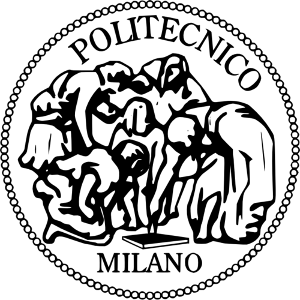
\includegraphics[width=0.5\textwidth]{images/polimi}
\end{figure}
\maketitle
\centering
A.Y. 2016/2017

Bolshakova Liubov, matr. 876911 

Gao Xiao, matr. 876265 

Kang Shuwen, matr. 876245

\end{titlepage}

\tableofcontents
\newpage
	
\section{INTRODUCTION}
	\subsection{Purpose}
	The integration test plan document is intended to describe how to accomplish the integration test. At first a high-level description of integration is provided to guide the specific testing. This document also includes the schedule and the processes of components which should be tested ,as well as the descriptions of the tools which are used.
	 
	\subsection{Scope}	
	
The total project is for design a software named \textsl{PowerEnJoy} which is an auto-servicing of cars for citizens. The aim of our software is not only supports the management of cars and provides a good quality of services to simplify the transportation, but also supports the payment and reservation services.
	\subsection{Glossary}
	\begin{itemize}
	\item Car: the cars that supplied for the car-sharing service in the \textsl{PowerEnJoy} system.
	\item Car information: the basic information that helps guests and users to make decisions, include the dump energy, location information, distance to the setting location, the passenger capacity.
	\item Starting position: the current position of user or the positions user input to start a ride.
	\item Available car: the car has dump energy more than 50% and be parked in the safe area.
	\item Available queue: a queue that maintains available cars 
	\item Sensors: the GPS and power plug sensor, weight sensor, display screen, battery sensor, door state sensor, locks of door in the car, and the sensor on the power grid. 
	\item System: the whole system, which include the electric devices and the \textsl{PowerEnJoy} system background.
	\item Ride: in this system, the ride process is started with ignite the engine and ended with all passengers leave the car.

	\end{itemize}
	
\newpage
\section{INTEGRATION STRATEGY}
	\subsection{Entry Criteria}
	In this section, we define some entry criteria, which are the conditions hold before the integration phase takes place. And these entry criteria are aimed at ensure the feasibility and correctness of the integration tests.	
	\begin{itemize}
		\item Reference Documents: The \textsl{Requirement Analysis and Specification Document} and \textsl{Design Document} are completed.
		\item Code: Every component to be tested is code completed, which means that all functionalities to be tested have been completely implemented.		
		\item Documentation: The documentation for each class and methods is fully provided and is understandable to testers.
		\item Unit Test: Every component is unit-tested by using JUnit and is bug free.
		\item Data: Test dataset is provided and functioned. 
		\item Tester: Manual testers are available. 
	\end{itemize}		
	\subsection{Elements to be integrated}
	In this section we identify the elements among which the integration test will be performed, by referring to the low-level components specified in the \textsl{Design Document}(as shown in Figure~\ref{fig-low}). For the sake of explicitness, we present the components according to the 3-tier architecture we designed in \textsl{Design Document}.
		\begin{figure}[H]
   			\centering
  			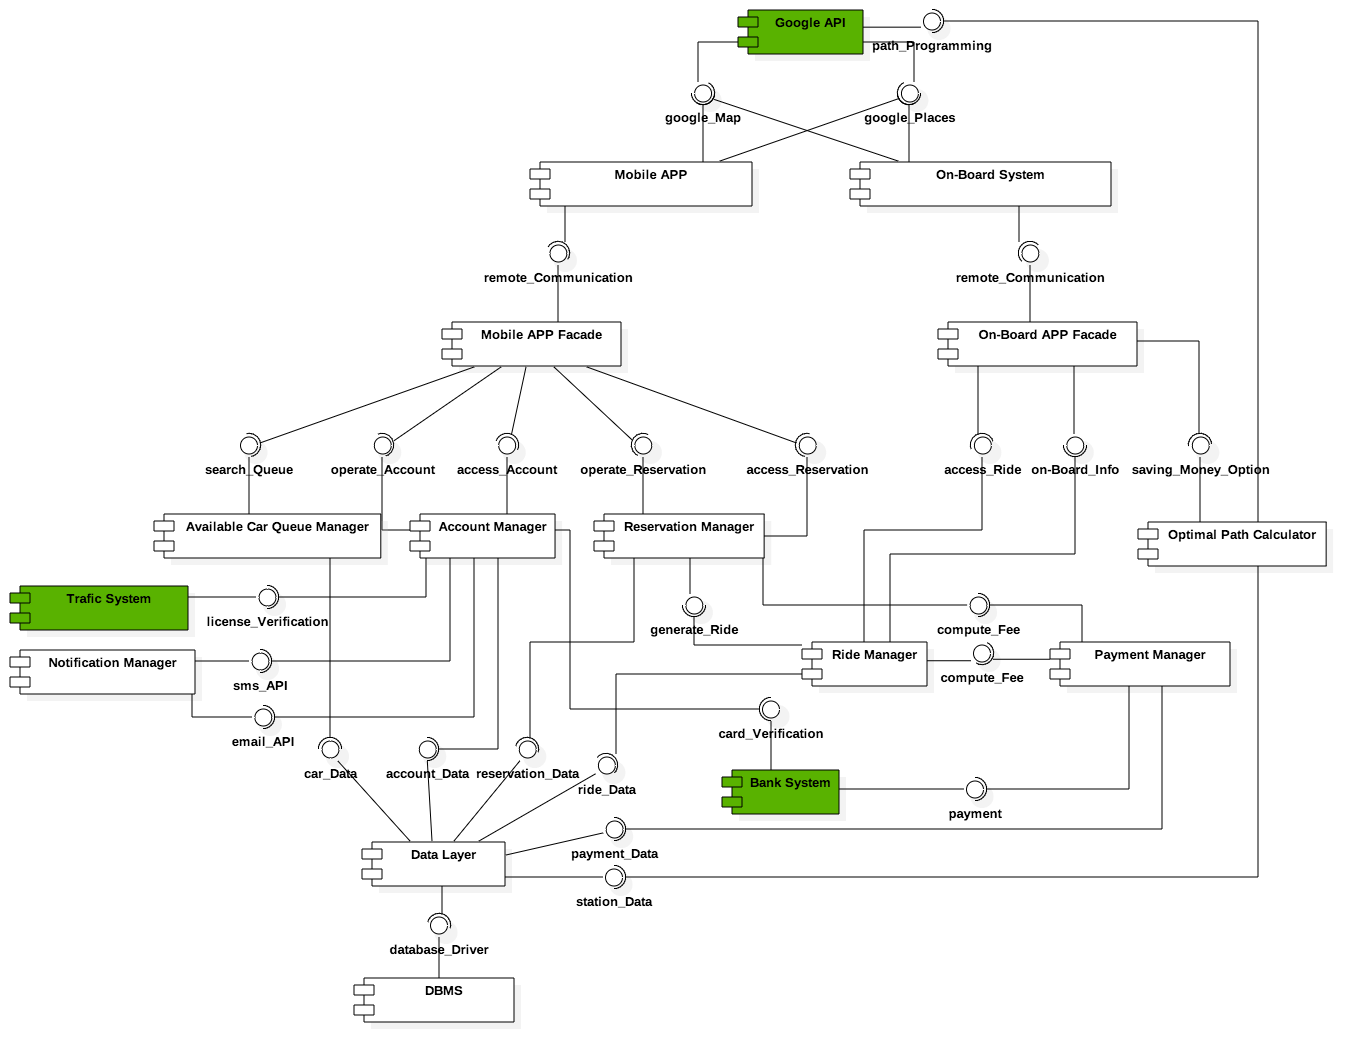
\includegraphics[width=\textwidth]{images/low_level_CD}
  	    		\caption{Low Level Component Diagram}\label{fig-low}
		\end{figure}
		
		\subsubsection{GUI Tier}
		Since the two components for presentation included in the \textsl{GUI} tier work independently, there are basically two elements to be integrated:
		\begin{itemize}
			\item Mobile APP component
			\item On-Board System component
		\end{itemize}
		\subsubsection{Application Tier}
		The \textsl{Application} tier provides the entire business logic of the system. We list all the elements to be integrated as follows:
		\begin{itemize}
			\item Mobile APP Facade
			\item On-Board APP Facade
			\item Available Queue Manager
			\item Account Manager 
			\item Reservation Manager
			\item Optimal Path Calculator
			\item Notification Manager
			\item Ride Manager
			\item Payment Manager
			\item Data Layer
			
		\end{itemize}
		\subsubsection{Data Tier}
		The \textsl{Data} tier contains the database used for data storage and the commercial database management system, namely the DBMS. These two components are coupled together and work properly according to the entry criteria we defined. For this reason, the only element to be integrated would be the DBMS component. 
		\subsubsection{External Components}
		Except of those components contained in the 3-Tier architecture, there is also a group of external components necessarily to be integrated into the \textsl{PowerEnJoy}, system, which are
		\begin{itemize}
			\item Google API,
			\item Bank System and
			\item Traffic System.
		\end{itemize}
			
	\subsection{Integration Test Strategy}
	In this section, we discuss about the \textbf{\textsl{bottom-up}} strategy, which we used for integration test, by explaining how we make the choice. 
	\subsubsection{System Partition}
	In order to better organize the test, we divide the entire system into three subsystems. Each subsystem contains several elements identified previously.
	\begin{itemize}
		\item Application Server: This subsystem works as the core of the entire system, and it contains all the elements we identified in the \textsl{Application Tier} and in the \textsl{External Components}.
		\item Mobile Client: This subsystem contains one of the components in \textsl{GUI Tier},namely the \textsl{Mobile APP}, as well as the \textsl{Google API} in the \textsl{External Components}.
		\item On-Board Client: Similar to the previous one, this subsystem includes the other components in \textsl{GUI Tier},which is the \textsl{Mobile APP}, together with the \textsl{Google API}.
	\end{itemize}
	\subsubsection{Integration Process}
	Since we have divided the entire system into three subsystems, our integration process will normally be performed in two phases:
	\begin{itemize}
		\item Local Integration: In this phase, we perform the integration of components within the subsystem.
		\item Overall Integration: In this phase, three individual subsystems will be integrated.
	\end{itemize}
	\subsubsection{Strategy Comparison}
	\begin{itemize}
		\item \textsl{Bottom-up strategy}: With this approach, we should start from the components in the bottom level,which have least dependency of other components and provide fundamental services to others, and add other components step by step. This approach is quite suitable to our system since we can reduce the total amount of needed stubs for integration accomplishment. 
		\item \textsl{Top-down strategy}: This kind of strategy is suggested in case of timing problem, because it is more focused on testing the functionalities provided to the end-user rather than considering about the real performance of low-level components.
		
		\item \textsl{Sandwich strategy}: This kind of strategy is more difficult to plan and implement in case of high-interdependent systems.
		
	\end{itemize}
	
	\subsection{Sequence of Components}
	In this section we discuss about the integration sequence for the \textsl{PowerEnJoy} system. Firstly, we preform the local integration individually in three subsystems that we have defined. And after that, we implement the overall integration for the entire system, namely carry out the integration between subsystems. Since the Application Server contains the most number of components to be integrated as well as a complex structure, our focus would be on the discussing about this particular subsystem. 
	\subsubsection{Application Server}
	To deal with the order of integration for such many components in this subsystem, we first illustrate the dependency relation between each component, which is shown in Figure~\ref{fig-dep}. And thanks to the dependency relation, we can simply distinguish six levels (as shown in Figure~\ref{fig-level}) for the Application Server, each of them contains several individual components which are independent with each other, so that the components within the same level can be tested in parallel. Between each two levels, there exists dependency, which means that the higher level cannot be integrated until the lower level works properly. 
		\begin{figure}[H]
   			\centering
  			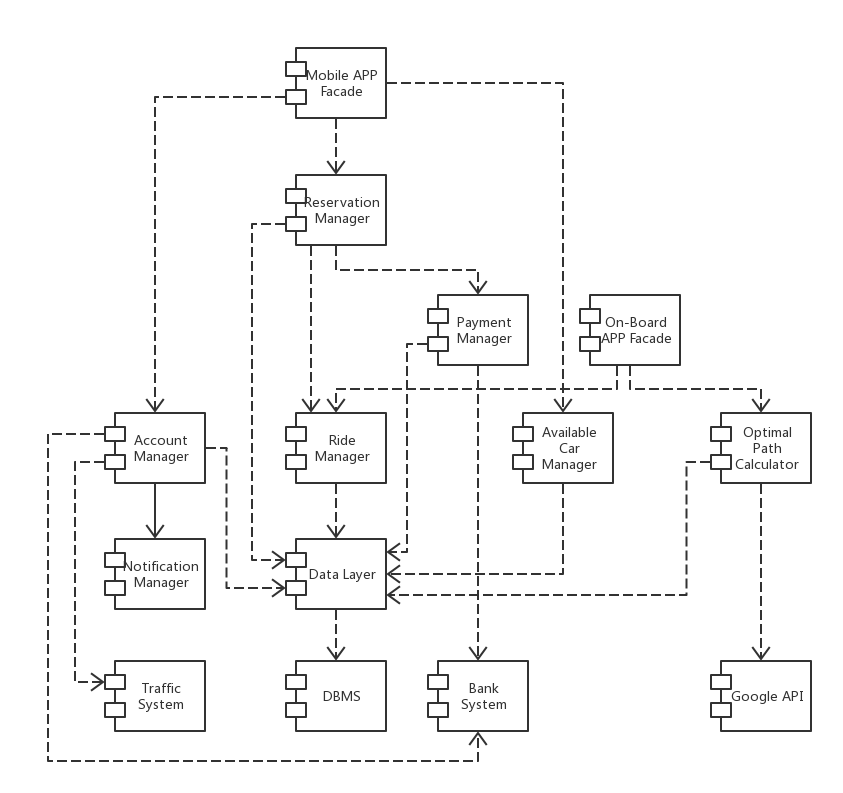
\includegraphics[width=\textwidth]{images/dep}
  	    		\caption{Dependency Relation}\label{fig-dep}
		\end{figure}
		\begin{figure}[H]
   			\centering
  			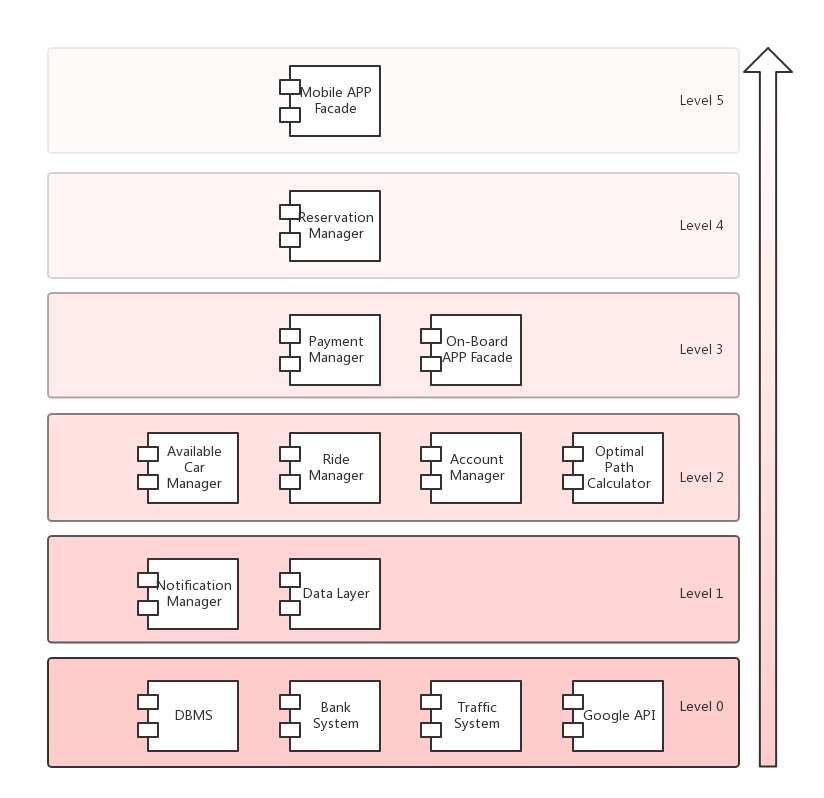
\includegraphics[width=\textwidth]{images/level}
  	    		\caption{Bottom-up Level}\label{fig-level}
		\end{figure}
	\subsubsection{Mobile Client}
	There are simply two components to be integrated within this subsystem. The dependency relation among them is illustrated in Figure~\ref{fig-depm}, according to which the integrated order might be decided.
		\begin{figure}[H]
   			\centering
  			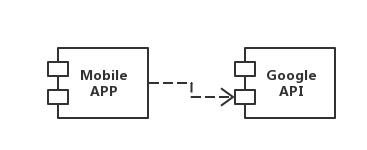
\includegraphics[width=\textwidth]{images/depm}
  	    		\caption{Dependency Relation}\label{fig-depm}
		\end{figure}
	
	\subsubsection{On-Board Client}
	Similar to the previous one, this subsystem also contains two components to be tested, and the sequence can be determined by means of Figure~\ref{fig-depo}.
		\begin{figure}[H]
   			\centering
  			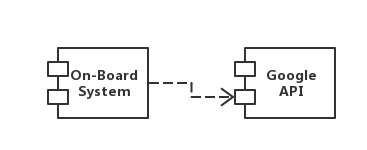
\includegraphics[width=\textwidth]{images/depo}
  	    		\caption{Dependency Relation}\label{fig-depo}
		\end{figure}
	\subsubsection{Overall System}
	In this phase, we have finished the individual subsystem testing and move on to the overall system integration. Since each subsystem is tested, we can assume that every functionality that we designed before has been implemented and works properly. Therefore the integration of subsystem would focus on the communication between each other. Again, we present the dependency relation of three subsystems in Figure~\ref{fig-depa}, and accordingly figure out the bottom-up level for them (as shown in Figure~\ref{fig-overall}. Not surprisingly, the subsystems within the same level can be tested in parallel. 
		\begin{figure}[H]
   			\centering
  			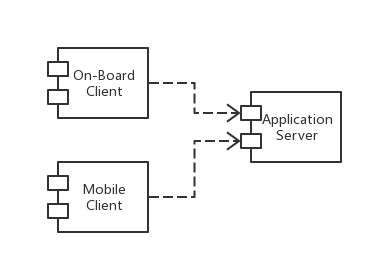
\includegraphics[width=\textwidth]{images/depa}
  	    		\caption{Dependency Relation}\label{fig-depa}
		\end{figure}
		\begin{figure}[H]
   			\centering
  			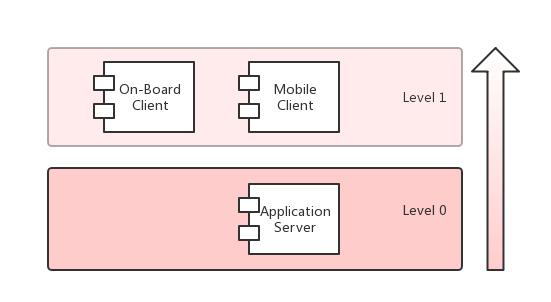
\includegraphics[width=\textwidth]{images/overall}
  	    		\caption{Overall Bottom-up Level}\label{fig-overall}
		\end{figure}
	\subsubsection{Integration Order}
	In this section we provide an alternative solution for the integration order of the entire system, which is illustrated in the table bellow. Notice that the integration order within the same bottom-up level might be decided arbitrarily since they are in parallel, therefore there exists numbers of solutions for the actual integration order which can be accepted. 	
\begin{table}[H]
\begin{center}
\renewcommand\arraystretch{1.5}
\begin{tabular}{|p{.5cm}|p{4cm}|p{4.5cm}|p{3.5cm}|}
 \hline
ID& Component&Dependency&Subsystem\\
 \hline
I01& DBMS&NULL&Application Server \\
 \hline
I02& Notification Manager&NULL&Application Server  \\
 \hline
I03& Data Layer&DBMS&Application Server \\
 \hline
I04& Available Car Manager&Data Layer&Application Server \\
 \hline
I05& Ride Manager&Data Layer&Application Server \\
 \hline
I06& Account Manager& Data Layer& Application Server \\
 \hline
I07& Optimal Path Calculator& Data Layer& Application Server \\
 \hline
 I08& Optimal Path Calculator& Google API& Application Server \\
 \hline
I09& Payment Manager&Data Layer&Application Server\\
 \hline
 I10& Payment Manager&Bank System&Application Server\\
 \hline
I11& On-Board APP Facade&Ride Manager&Application Server \\
 \hline
 I12& On-Board APP Facade&Optimal Path Calculator&Application Server \\
 \hline
I13& Reservation Manager&Data Layer&Application Server\\
 \hline
 I14& Reservation Manager&Ride Manager&Application Server\\
 \hline
 I15& Reservation Manager&Payment Manager&Application Server\\
 \hline
 I16& Mobile APP Facade&Account Manager&Application Server \\
 \hline
 I17&  Mobile APP Facade&Reservation Manager&Application Server\\
 \hline
 I18&  Mobile APP Facade&Available Car Manager&Application Server\\
 \hline
 I19& On-Board System&Google API& On-Board Client \\
 \hline
 I20&  On-Board System&On-Board APP Facade&On-Board Client\\
 \hline
 I21&  Mobile APP&Google API& Mobile Client\\
 \hline
 I22&  Mobile APP&Mobile APP Facade& Mobile Client\\
 \hline
\end{tabular}
\caption{Integration Order}
\end{center}
\end{table}	

	
\newpage	
\section{INDIVIDUAL STEP AND TEST DESCRIPTION}
For a better understanding we are going to show a high-level description of the integration tests that will be performed on PowerEnJoy system. The bottom-up strategy choice implies the use of drivers: every driver is associated to a specific software component, and is used to simulate the input coming from a already tested component,this ensure us to get rid of factors which are surely be right, then we can focus on the factors only associated to the testing component.
The following tables are structured as:
\begin{itemize}
	\item Test Case ID: an identifier for the analyzed integration test.
	\item Test Items: the couple of involved components; the arrow represent the «depend on» relationship. 
 	\item Input Specification: the high-level description of the input coming from the right element of the couple specified at Test Item row.
	\item Output Specification: the high-level description of the expected output of the input above.
	\item Environmental Needs: the conditions under which the test can be executed, in terms of:
	\begin{itemize}
		\item already performed tests
		\item already implemented drivers
	\end{itemize}
\end{itemize}

	\subsection{Application Server}
		\subsubsection{DBMS Integration Test}
\begin{table}[H] 
\begin{center}
\renewcommand\arraystretch{1.5}
\begin{tabular}{|p{5cm}|p{7cm}|}
 \hline
\textbf{Test Case ID}& I01\\
 \hline
\textbf{Test Item}&DBMS\\
 \hline
\textbf{Input Specification}&The test of DBMS is execute the data search function from every GUI in users' terminal.\\
 \hline
\textbf{Output Specification}&Check if the correct data was responded according to the SQL search in the database.\\
 \hline
 \textbf{Environmental Needs}&The DBMS is connected with the system, the database Driver already been implemented.\\
 \hline
\end{tabular}
\end{center}
\end{table}		
		\subsubsection{Notification Manager Integration Test}
\begin{table}[H] 
\begin{center}
\renewcommand\arraystretch{1.5}
\begin{tabular}{|p{5cm}|p{7cm}|}
 \hline
\textbf{Test Case ID}& I02\\
 \hline
\textbf{Test Item}&Notification Manager\\
 \hline
\textbf{Input Specification}&Simulate the Notification Manager component, the test should also cover the exceptional and edge cases related to the sms API and email API interface.\\
 \hline
\textbf{Output Specification}&Check if the email addresses or telephone numbers can get the present information.\\
 \hline
 \textbf{Environmental Needs}&The Notification Manager should connected to the system.\\
 \hline
\end{tabular}
\end{center}
\end{table}		
		\subsubsection{Data Layer Integration Test}
\begin{table}[H] 
\begin{center}
\renewcommand\arraystretch{1.5}
\begin{tabular}{|p{5cm}|p{7cm}|}
 \hline
\textbf{Test Case ID}& I03\\
 \hline
\textbf{Test Item}&Data Layer $\rightarrow$ DBMS\\
 \hline
\textbf{Input Specification}&Manipulate the DBMS with the data from the Data Layer or search the data in DBMS by the requests from Data Layer.\\
 \hline
\textbf{Output Specification}&Check if the correct methods are invoked, along with the correct value and parameter types.\\
 \hline
 \textbf{Environmental Needs}&The DBMS must have been already implemented.\\
 \hline
\end{tabular}
\end{center}
\end{table}		
		\subsubsection{Available Car Manager Integration Test}
		\begin{table}[H] 
\begin{center}
\renewcommand\arraystretch{1.5}
\begin{tabular}{|p{5cm}|p{7cm}|}
 \hline
\textbf{Test Case ID}& I04\\
 \hline
\textbf{Test Item}&Available Car Manager $\rightarrow$ Data Layer\\
 \hline
\textbf{Input Specification}&Simulate the Available Car Manager component with the input from the Data layer,the test should also cover the exceptional and edge cases related to the search Queue interface and car Data interface.\\
 \hline
\textbf{Output Specification}&Check if the correct methods are used;
Check if the parameters are in the correct type according to the methods, as well as the correctness of values.\\
 \hline
 \textbf{Environmental Needs}&The Data Layer driver must have been already implemented.\\
 \hline
\end{tabular}
\end{center}
\end{table}		
		\subsubsection{Ride Manager Integration Test}
		\begin{table}[H] 
\begin{center}
\renewcommand\arraystretch{1.5}
\begin{tabular}{|p{5cm}|p{7cm}|}
 \hline
\textbf{Test Case ID}& I05\\
 \hline
\textbf{Test Item}&Ride Manager$\rightarrow$ Data Layer\\
 \hline
\textbf{Input Specification}&Simulate the Ride Manager component with the input from the Data layer, the test should also cover the exceptional and edge cases related to the access Ride and access Fee Interface and ride Data interface.\\
 \hline
\textbf{Output Specification}&Check if the correct methods are used;
Check if the parameters are in the correct type according to the methods, as well as the correctness of values.\\
 \hline
 \textbf{Environmental Needs}&The Data Layer driver must have been already implemented.\\
 \hline
\end{tabular}
\end{center}
\end{table}		
		\subsubsection{Account Manager Integration Test}
		\begin{table}[H] 
\begin{center}
\renewcommand\arraystretch{1.5}
\begin{tabular}{|p{5cm}|p{7cm}|}
 \hline
\textbf{Test Case ID}& I06\\
 \hline
\textbf{Test Item}&Account Manager $\rightarrow$Data Layer\\
 \hline
\textbf{Input Specification}&Simulate the Account Manager component with the input from the Data layer, the test should also cover the exceptional and edge cases related to the operate Account and access Account Interface and account Data interface.\\
 \hline
\textbf{Output Specification}&Check if the correct methods are used;
Check if the parameters are in the correct type according to the methods, as well as the correctness of values.\\
 \hline
 \textbf{Environmental Needs}&The Data Layer driver must have been already implemented.\\
 \hline
\end{tabular}
\end{center}
\end{table}		
		\subsubsection{Optimal Path Calculator Integration Test}
		\begin{table}[H] 
\begin{center}
\renewcommand\arraystretch{1.5}
\begin{tabular}{|p{5cm}|p{7cm}|}
 \hline
\textbf{Test Case ID}& I07\\
 \hline
\textbf{Test Item}&Optimal Path Calculator $\rightarrow$Data Layer\\
 \hline
\textbf{Input Specification}&Simulate the Optimal Path Calculator component with the input from the Data layer, the test should also cover the exceptional and edge cases related to the saving Money Option Interface and station Data interface.\\
 \hline
\textbf{Output Specification}&Check if the correct methods are used;
Check if the parameters are in the correct type according to the methods, as well as the correctness of values.\\
 \hline
 \textbf{Environmental Needs}&The Data Layer driver must have been already implemented.\\
 \hline
\end{tabular}
\end{center}
\end{table}		
\begin{table}[H] 
\begin{center}
\renewcommand\arraystretch{1.5}
\begin{tabular}{|p{5cm}|p{7cm}|}
 \hline
\textbf{Test Case ID}& I08\\
 \hline
\textbf{Test Item}&Optimal Path Calculator $\rightarrow$Google API\\
 \hline
\textbf{Input Specification}&Simulate the Optimal Path component with the input from the Google API, the test should also cover the exceptional and edge cases related to the saving Money Option Interface and google path Programming interface.\\
 \hline
\textbf{Output Specification}&Check if the correct methods are used;
Check if the parameters are in the correct type according to the methods, as well as the correctness of values.\\
 \hline
 \textbf{Environmental Needs}&The Google API must have been already connected to the system.\\
 \hline
\end{tabular}
\end{center}
\end{table}		
		\subsubsection{Payment Manager Integration Test}
		\begin{table}[H] 
\begin{center}
\renewcommand\arraystretch{1.5}
\begin{tabular}{|p{5cm}|p{7cm}|}
 \hline
\textbf{Test Case ID}& I09\\
 \hline
\textbf{Test Item}&Payment Manager$\rightarrow$ Data Layer\\
 \hline
\textbf{Input Specification}&Simulate the Payment Manager component with the input from the Data layer, the test should also cover the exceptional and edge cases related to the payment Interface and payment Data interface.\\
 \hline
\textbf{Output Specification}&Check if the correct methods are used;
Check if the parameters are in the correct type according to the methods, as well as the correctness of values.\\
 \hline
 \textbf{Environmental Needs}&The Data Layer driver must have been already implemented.\\
 \hline
\end{tabular}
\end{center}
\end{table}		
\begin{table}[H] 
\begin{center}
\renewcommand\arraystretch{1.5}
\begin{tabular}{|p{5cm}|p{7cm}|}
 \hline
\textbf{Test Case ID}& I10\\
 \hline
\textbf{Test Item}&Payment Manager $\rightarrow$Bank System\\
 \hline
\textbf{Input Specification}&Simulate the Payment Manager component with the input from the Bank System, the test should also cover the exceptional and edge cases related to the card Verification Interface,payment interface.\\
 \hline
\textbf{Output Specification}&Check if the correct methods are used;
Check if the parameters are in the correct type according to the methods, as well as the correctness of values.\\
 \hline
 \textbf{Environmental Needs}&The Bank System must have been already connected with the system.\\
 \hline
\end{tabular}
\end{center}
\end{table}		
		\subsubsection{On-Board APP Facade Integration Test}
		\begin{table}[H] 
\begin{center}
\renewcommand\arraystretch{1.5}
\begin{tabular}{|p{5cm}|p{7cm}|}
 \hline
\textbf{Test Case ID}& I11\\
 \hline
\textbf{Test Item}&On-Board APP Facade $\rightarrow$Ride Manager\\
 \hline
\textbf{Input Specification}&Simulate the On-Board APP Facade component with the input from the Ride Manager, the test should also cover the exceptional and edge cases related to the On-Board APP Facade Interface.\\
 \hline
\textbf{Output Specification}&Check if the correct methods are used;
Check if the parameters are in the correct type according to the methods, as well as the correctness of values.\\
 \hline
 \textbf{Environmental Needs}&The Ride Manager driver must have been already implemented.\\
 \hline
\end{tabular}
\end{center}
\end{table}		
\begin{table}[H] 
\begin{center}
\renewcommand\arraystretch{1.5}
\begin{tabular}{|p{5cm}|p{7cm}|}
 \hline
\textbf{Test Case ID}& I12\\
 \hline
\textbf{Test Item}&On-Board System Facade $\rightarrow$Optimal Path Calculator\\
 \hline
\textbf{Input Specification}&Simulate the On-Board System Facade component with the input from the Optimal Path Calculator. the test should also cover the exceptional and edge cases related to the on-Board Info Interface, saving Money Option interface and remote Communication interface.\\
 \hline
\textbf{Output Specification}&Check if the correct methods are used;
Check if the parameters are in the correct type according to the methods, as well as the correctness of values.\\
 \hline
 \textbf{Environmental Needs}&The Optimal Path Calculator driver must have been already implemented.\\
 \hline
\end{tabular}
\end{center}
\end{table}		
		\subsubsection{Reservation Manager Integration Test}
		\begin{table}[H] 
\begin{center}
\renewcommand\arraystretch{1.5}
\begin{tabular}{|p{5cm}|p{7cm}|}
 \hline
\textbf{Test Case ID}& I13\\
 \hline
\textbf{Test Item}&Reservation Manager$\rightarrow$ Data Layer\\
 \hline
\textbf{Input Specification}&Simulate the Reservation Manager component with the input from the Data Layer. the test should also
cover the exceptional and edge cases related to the operate Reservation Interface,access Reservation interface.\\
 \hline
\textbf{Output Specification}&Check if the correct methods are used;
Check if the parameters are in the correct type according to the methods, as well as the correctness of values.\\
 \hline
 \textbf{Environmental Needs}&The Data Layer driver must have been already implemented.\\
 \hline
\end{tabular}
\end{center}
\end{table}		
\begin{table}[H] 
\begin{center}
\renewcommand\arraystretch{1.5}
\begin{tabular}{|p{5cm}|p{7cm}|}
 \hline
\textbf{Test Case ID}& I14\\
 \hline
\textbf{Test Item}&Reservation Manager $\rightarrow$Ride Manager\\
 \hline
\textbf{Input Specification}&Simulate the Reservation Manager component with the input from the Ride Manager. the test should also cover the exceptional and edge cases related to the Reservation Manager Interface and Ride Manager Interface.\\
 \hline
\textbf{Output Specification}&Check if the correct methods are used;
Check if the parameters are in the correct type according to the methods, as well as the correctness of values.\\
 \hline
 \textbf{Environmental Needs}&The Ride Manager driver must have been already implemented.\\
 \hline
\end{tabular}
\end{center}
\end{table}		
\begin{table}[H] 
\begin{center}
\renewcommand\arraystretch{1.5}
\begin{tabular}{|p{5cm}|p{7cm}|}
 \hline
\textbf{Test Case ID}& I15\\
 \hline
\textbf{Test Item}&Reservation Manager $\rightarrow$Payment Manager\\
 \hline
\textbf{Input Specification}&Simulate the Reservation Manager component with the input from the Payment Manager. the test should also cover the exceptional and edge cases related to the Reservation Manager Interface and Payment Manager interface.\\
 \hline
\textbf{Output Specification}&Check if the correct methods are used;
Check if the parameters are in the correct type according to the methods, as well as the correctness of values.\\
 \hline
 \textbf{Environmental Needs}&The Payment Manager driver must have been already implemented.\\
 \hline
\end{tabular}
\end{center}
\end{table}		
		\subsubsection{Mobile APP Facade Integration Test}
		\begin{table}[H] 
\begin{center}
\renewcommand\arraystretch{1.5}
\begin{tabular}{|p{5cm}|p{7cm}|}
 \hline
\textbf{Test Case ID}& I16\\
 \hline
\textbf{Test Item}&Mobile APP Facade $\rightarrow$Account Manager\\
 \hline
\textbf{Input Specification}&Simulate the Mobile APP Facade component with the input from the Account Manager. the test should also cover the exceptional and edge cases related to the
Account Manager Interface and .\\
 \hline
\textbf{Output Specification}&Check if the correct methods are used;
Check if the parameters are in the correct type according to the methods, as well as the correctness of values.
Environmental Needs\\
 \hline
 \textbf{Environmental Needs}&The Account Manager driver must have been already implemented.\\
 \hline
\end{tabular}
\end{center}
\end{table}		
\begin{table}[H] 
\begin{center}
\renewcommand\arraystretch{1.5}
\begin{tabular}{|p{5cm}|p{7cm}|}
 \hline
\textbf{Test Case ID}& I17\\
 \hline
\textbf{Test Item}&Mobile APP Facade $\rightarrow$Reservation Manage\\
 \hline
\textbf{Input Specification}&Simulate the Mobile APP Facade component with the input from the Reservation Manager. the test should also cover the exceptional and edge cases related to the Reservation Manager Interface and Mobile APP Facade interface.\\
 \hline
\textbf{Output Specification}&Check if the correct methods are used;
Check if the parameters are in the correct type according to the methods, as well as the correctness of values.\\
 \hline
 \textbf{Environmental Needs}&The Reservation Manager driver must have been already implemented.\\
 \hline
\end{tabular}
\end{center}
\end{table}		
\begin{table}[H] 
\begin{center}
\renewcommand\arraystretch{1.5}
\begin{tabular}{|p{5cm}|p{7cm}|}
 \hline
\textbf{Test Case ID}& I18\\
 \hline
\textbf{Test Item}&Mobile APP Facade $\rightarrow$Available Car Manager\\
 \hline
\textbf{Input Specification}&Simulate the Mobile APP Facade component with the input from the Available Car Manager. the test should also cover the exceptional and edge cases related to the Available Car Manager Interface and Mobile APP Facade interface.\\
 \hline
\textbf{Output Specification}&Check if the correct methods are used;
Check if the parameters are in the correct type according to the methods, as well as the correctness of values.\\
 \hline
 \textbf{Environmental Needs}&The Available Car Manager driver must have been already implemented.\\
 \hline
\end{tabular}
\end{center}
\end{table}		
	
	\subsection{On-Board Client}
		\subsubsection{On-Board System Integration Test}
		\begin{table}[H] 
\begin{center}
\renewcommand\arraystretch{1.5}
\begin{tabular}{|p{5cm}|p{7cm}|}
 \hline
\textbf{Test Case ID}& I19\\
 \hline
\textbf{Test Item}&On-Board System $\rightarrow$Google API\\
 \hline
\textbf{Input Specification}&Simulate the On-Board System component with the input from the Google API. the test should also cover the exceptional and edge cases related to the On- Board System interface,Google API Interface.\\
 \hline
\textbf{Output Specification}&Check if the correct methods are used;
Check if the parameters are in the correct type according to the methods, as well as the correctness of values.\\
 \hline
 \textbf{Environmental Needs}&The Goolge API must have been already implemented.\\
 \hline
\end{tabular}
\end{center}
\end{table}		
\begin{table}[H] 
\begin{center}
\renewcommand\arraystretch{1.5}
\begin{tabular}{|p{5cm}|p{7cm}|}
 \hline
\textbf{Test Case ID}& I20\\
 \hline
\textbf{Test Item}&On-Board System$\rightarrow$ On-Board APP Facade\\
 \hline
\textbf{Input Specification}&Simulate the On-Board System component with the input from the On-Board APP Facade. the test should also cover the exceptional and edge cases related to the Reservation Manager Interface.\\
 \hline
\textbf{Output Specification}&Check if the correct methods are used;
Check if the parameters are in the correct type according to the methods, as well as the correctness of values.\\
 \hline
 \textbf{Environmental Needs}&The On-Board APP Facade driver must have been already implemented.\\
 \hline
\end{tabular}
\end{center}
\end{table}		
	
	\subsection{Mobile Client}
		\subsubsection{Mobile APP Integration Test}
		\begin{table}[H] 
\begin{center}
\renewcommand\arraystretch{1.5}
\begin{tabular}{|p{5cm}|p{7cm}|}
 \hline
\textbf{Test Case ID}& I21\\
 \hline
\textbf{Test Item}&Mobile APP $\rightarrow$ Google API\\
 \hline
\textbf{Input Specification}&Simulate the Mobile APP component with the input from the Google API. the test should also cover the exceptional and edge cases related to the Reservation Manager Interface.\\
 \hline
\textbf{Output Specification}&Check if the correct methods are used;
Check if the parameters are in the correct type according to the methods, as well as the correctness of values.\\
 \hline
 \textbf{Environmental Needs}&The Google API must have been already connected to the system.\\
 \hline
\end{tabular}
\end{center}
\end{table}		


\begin{table}[H] 
\begin{center}
\renewcommand\arraystretch{1.5}
\begin{tabular}{|p{5cm}|p{7cm}|}
 \hline
\textbf{Test Case ID}& I22\\
 \hline
\textbf{Test Item}&Mobile APP $\rightarrow$ Mobile APP Facade\\
 \hline
\textbf{Input Specification}&Simulate the Mobile APP component with the input from the Mobile APP Facade. the test should also cover the exceptional and edge cases related to the Reservation Manager Interface.\\
 \hline
\textbf{Output Specification}&Check if the correct methods are used;
Check if the parameters are in the correct type according to the methods, as well as the correctness of values.\\
 \hline
 \textbf{Environmental Needs}&The Mobile APP Facade driver must have been already implemented.\\
 \hline
\end{tabular}
\end{center}
\end{table}		


\newpage
\section{TOOLS AND TEST EQUIPMENT REQUIRED}
	\subsection{Tools}
	In order to make sure that each components within the system works appropriately, we use some effective testing tools, which will be discussed in detail in the next few paragraphs.
		\subsubsection{JUnit}
		JUnit is a unit testing framework for the Java programming language. It has a very important development in test-driven field. We make the decision to use it mainly because that it simplifies the unit testing of components. 
		\subsubsection{Arquillian}
		Arquillian is a JUnit-based test framework. Indeed Arquillian represents an optimal solution in a such context where more components have to be tested and integrated among them. Thanks to this testing tool, the integration tests and the functional tests could be as simple as unit tests. In accordance with the design document, Java EE will be the main framework for the development of our system. That's why Arquillian should be the best solution in these case in which the integration among multiple enterprise components has to be tested.
		\subsubsection{Database}
		\begin{itemize}
		\item MySQL Database
		\item MySQL Connector/J 5.1.40
		\end{itemize}				
		
	\subsection{Test Equipment}
	These testing devices would be used to test both the Mobile Application and the On-Board Application. it is also should be noted that, the testing devices should be as general as possible. The range of the testing devices selection, should cover the wildest range of the possible configuration.

In fact, for satisfying the most general case, we should consider to survey the smartphone marker. If we want to get the most general testing result, we should use the most widely used devices, in order to better reflect the typical usage scenarios we would encounter in the real operating environment.
		\subsubsection{Mobile Phone}
		For Mobile Client testing: 
			\begin{itemize}
			\item At least one Android smart phone, which is running Android operation system(version 4.0 ( Ice Cream Sandwich) or higher).
			\item At least one IOS smart phone, which is running IOS operating system(version 7.1.2 or higher).
			\item At least one Windows smart phone, which is running Windows operating system.
			\end{itemize}					
		
		\subsubsection{On-Board Embedded System}
		On-Board physical equipment which is normally provided on the \textsl{PowerEnJoy} car.
		


\newpage
\section{PROGRAM DRIVERS AND TEST DATA REQUIRED}
	\subsection{Program Drivers and Stubs}
	In our testing phase, we use a bottom-up approach to compose the components of the system. Therefore, we also use the bottom-up framework to compose the integration and testing.

In order to complete the testing of a single component in the Application Server subsystem, we are going to use a number of drivers to drive each component for simulating the real system. What's more, we need the drivers to perform the necessary function call for testing.

As for the other two subsystems, On-Board Client and Mobile Client, we need proper stubs to provide function call response. Thanks to the stubs, each of our three subsystems can be tested individually. 

In the following paragraph we list the drivers and stubs which are used during the testing, and provide further discussion about them.
	\begin{itemize}
	\item \textbf{DBMS driver}
	
	This driver is in charge of performing data exchange with DBMS, in order to test the integration between DBMS and the Database.
	\item \textbf{Data Layer driver}
	
	This driver is designed to invoke the methods provided by Data Layer, aiming at checking the integration between Data Layer and it's sub-level components.
	\item \textbf{Notification Manager driver}
	
	For the aim of testing the Notification Manager, we need this driver to simulate a notification call to the Notification Manager, so as to check the performance.
	\item \textbf{Available Car Manager driver}
	
	This driver is in charge of invoking the methods provided by Available Car Manager, testing the integration state to the sub-level components.
	\item \textbf{Ride Manager driver}
	
	The main purpose of this driver is to simulate a ride generate call, in order to invoke the methods within Ride Manager. By checking the response from Ride Manager we can observe the integration status between Ride Manager and it's sub-level components.
	\item \textbf{Account Manager driver}
	
	This driver is designed to perform data exchange with Account Manager, aiming at testing the integration of Account Manager together with it's sub-level components.
	\item \textbf{Optimal Path Calculator driver}
	
	This driver basically provides position informations to Optimal Path Calculator, in order to invoke the algorithm so as to test it's integration with the Data Layer.
	\item \textbf{Payment Manager driver}
	
	This driver is in charge of checking the integration state of Payment Manager with lower level components by simulating a payment call to Payment Manager.
	\item \textbf{On-Board APP Facade driver}
	
	This driver simulates the function call from On-Board System, and hence it tests the integration of On-Board APP Facade with lower level components. 
	\item \textbf{Reservation Manager driver}
	
	This driver is designed to perform data exchange with Reservation Manager, aiming at testing the integration of Reservation Manager together with it's sub-level components.
	\item \textbf{Mobile APP Facade driver}
	
	This driver simulates the function call from Mobile APP, and hence it tests the integration of Mobile APP Facade with lower level components. 
	\item \textbf{On-Board client stub}
	
	This stub simulates the response of On-Board APP Facade, aiming at checking the information display and interaction performance on the On-Board System.
	\item \textbf{Mobile Client stub}
	
	This stub is designed to provide simulated response from Mobile APP Facade, for the aim of checking the information display and interaction performance on the Mobile APP.
	\end{itemize}
	
	\subsection{Test Database}
	In order to perform the tests a database configured as specified in the design document must be used. This database might contain dummy data, crafted in a way and number that allow for exhaustive tests on the data layer. The structure of the test database must comply with the specification of the E-R diagram provided in the design phase, which is shown in Figure~\ref{fig-ER}.
\begin{figure}[H]
   			\centering
  			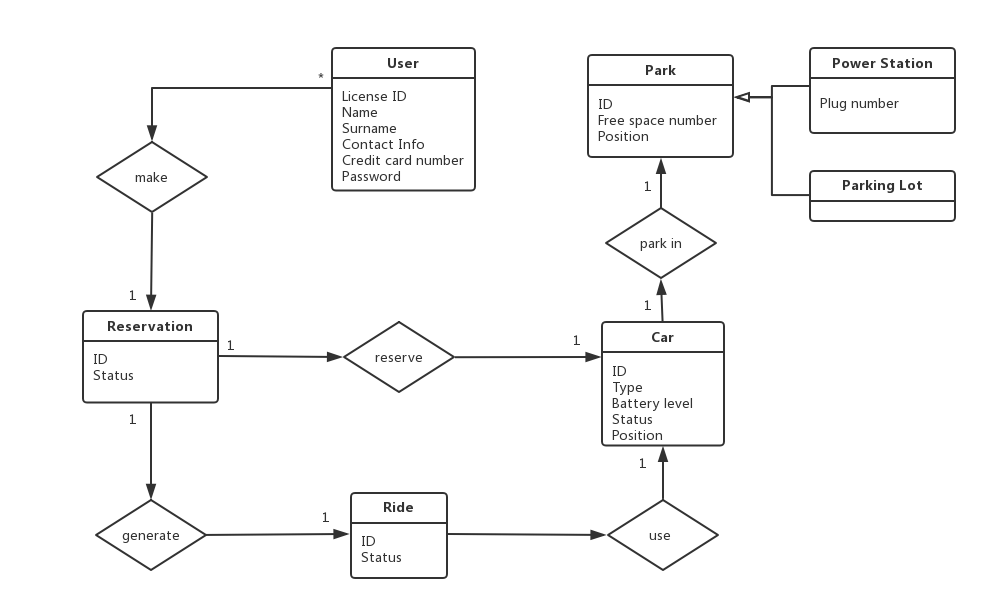
\includegraphics[width=\textwidth]{images/ER}
  	    		\caption{ER-diagram}\label{fig-ER}
		\end{figure}
\newpage
\section{EFFORT SPENT}

\renewcommand\arraystretch{2}
\begin{tabular}{| p{5cm}| p{7cm}|}
 \hline
Gao Xiao& 20 Hours \\
 \hline
Kang Shuwen& 25 Hours \\
 \hline
Liubov Bolshakova& 10 Hours \\
 \hline

\end{tabular}

\newpage
\section{REFERENCES}
	\subsection{Reference Documents}
	\begin{itemize}
		\item Specification Document Assignments AA 2016-2017
		\item RASD
		\item DD
	\end{itemize}
	\subsection{Used Tools}
	The tools used to creat this document are:
	\begin{itemize}
		\item UMLStar: for UML models
		\item Github: for version control
		\item Latex: for typesetting
		\item ProcessOn: for network diagram
		 
	\end{itemize}

\newpage
	
\end{document}